\documentclass[tikz, border=10pt]{standalone}
\usepackage{tikz}
\usetikzlibrary{shapes.geometric, arrows.meta, positioning, fit, backgrounds}

\definecolor{grucolor}{RGB}{52, 120, 190}
\definecolor{mhacolor}{RGB}{34, 150, 100}
\definecolor{mlpcolor}{RGB}{190, 80, 50}
\definecolor{normcolor}{RGB}{120, 90, 170}
\definecolor{addcolor}{RGB}{80, 80, 80}
\definecolor{arrowcolor}{RGB}{60, 60, 60}
\definecolor{bgblock}{RGB}{245, 248, 255}

\tikzset{
  block/.style={
    rectangle, rounded corners=4pt,
    minimum width=3.2cm, minimum height=0.75cm,
    text centered, font=\small\bfseries,
    draw, thick
  },
  normblock/.style={
    block,
    fill=normcolor!20, draw=normcolor!70,
    text=normcolor!80!black
  },
  grublock/.style={
    block,
    fill=grucolor!20, draw=grucolor!70,
    text=grucolor!80!black
  },
  mhablock/.style={
    block,
    fill=mhacolor!20, draw=mhacolor!70,
    text=mhacolor!80!black
  },
  mlpblock/.style={
    block,
    fill=mlpcolor!20, draw=mlpcolor!70,
    text=mlpcolor!80!black
  },
  addblock/.style={
    circle, minimum size=0.55cm,
    text centered, font=\small\bfseries,
    fill=addcolor!15, draw=addcolor!60,
    text=addcolor
  },
  ioblock/.style={
    rectangle, rounded corners=2pt,
    minimum width=3.2cm, minimum height=0.6cm,
    text centered, font=\small,
    fill=gray!15, draw=gray!50
  },
  arr/.style={
    -{Stealth[length=5pt]}, thick, color=arrowcolor
  },
  skiparr/.style={
    -{Stealth[length=5pt]}, thick, color=addcolor!70, dashed
  }
}

\begin{document}
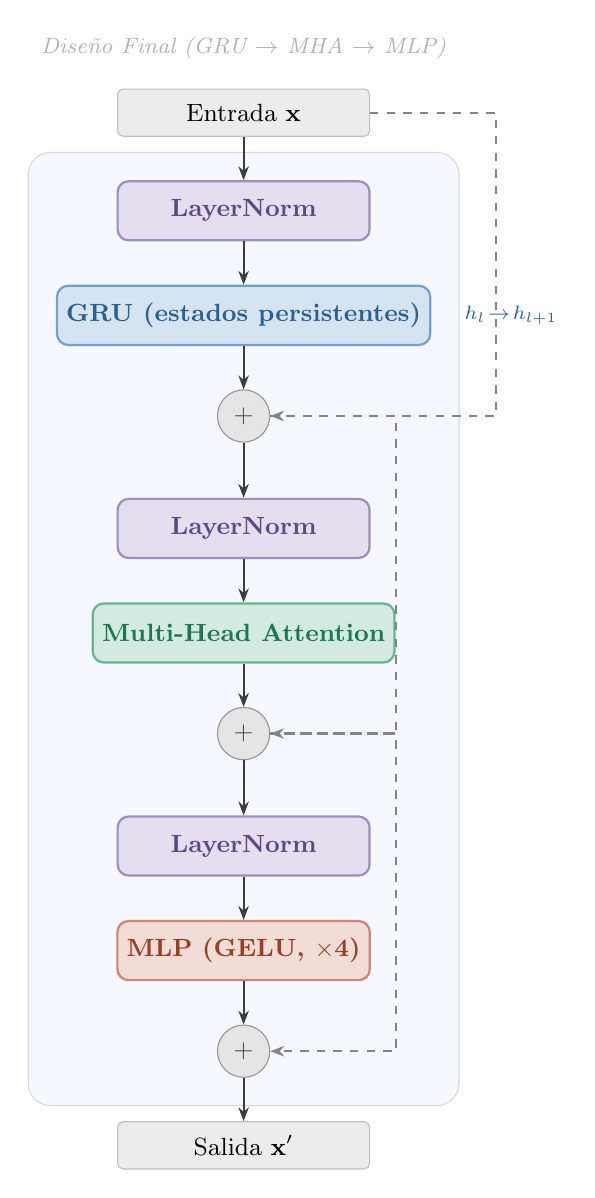
\begin{tikzpicture}[node distance=0.55cm]

  % ── Block title ────────────────────────────────────────────
  \node[font=\footnotesize\itshape, text=gray!60] (title) {Diseño Final (GRU $\to$ MHA $\to$ MLP)};

  % ── Input ──────────────────────────────────────────────────
  \node[ioblock, below=0.25cm of title] (input) {Entrada $\mathbf{x}$};

  % ── GRU sub-block ──────────────────────────────────────────
  \node[normblock, below=of input]           (ln1)  {LayerNorm};
  \node[grublock,  below=of ln1]             (gru)  {GRU (estados persistentes)};
  \node[addblock,  below=of gru]             (add1) {$+$};

  % ── MHA sub-block ──────────────────────────────────────────
  \node[normblock, below=0.7cm of add1]      (ln2)  {LayerNorm};
  \node[mhablock,  below=of ln2]             (mha)  {Multi-Head Attention};
  \node[addblock,  below=of mha]             (add2) {$+$};

  % ── MLP sub-block ──────────────────────────────────────────
  \node[normblock, below=0.7cm of add2]      (ln3)  {LayerNorm};
  \node[mlpblock,  below=of ln3]             (mlp)  {MLP (GELU, $\times$4)};
  \node[addblock,  below=of mlp]             (add3) {$+$};

  % ── Output ─────────────────────────────────────────────────
  \node[ioblock, below=of add3]              (output) {Salida $\mathbf{x}'$};

  % ── Main flow arrows ───────────────────────────────────────
  \draw[arr] (input)  -- (ln1);
  \draw[arr] (ln1)    -- (gru);
  \draw[arr] (gru)    -- (add1);
  \draw[arr] (add1)   -- (ln2);
  \draw[arr] (ln2)    -- (mha);
  \draw[arr] (mha)    -- (add2);
  \draw[arr] (add2)   -- (ln3);
  \draw[arr] (ln3)    -- (mlp);
  \draw[arr] (mlp)    -- (add3);
  \draw[arr] (add3)   -- (output);

  % ── Residual skip connections ───────────────────────────────
  \draw[skiparr] (input.east) -- ++(1.6,0) |- (add1.east);
  \draw[skiparr] (add1.east)  -- ++(1.6,0) |- (add2.east);
  \draw[skiparr] (add2.east)  -- ++(1.6,0) |- (add3.east);

  % ── Background block border ─────────────────────────────────
  \begin{scope}[on background layer]
    \node[
      fill=bgblock, draw=gray!30, rounded corners=8pt,
      inner sep=10pt,
      fit=(ln1)(gru)(add1)(ln2)(mha)(add2)(ln3)(mlp)(add3)
    ] (border) {};
  \end{scope}

  % ── Hidden state annotation ──────────────────────────────────
  \node[
    font=\scriptsize, text=grucolor!80!black,
    right=0.3cm of gru, align=left
  ] {$h_l \!\rightarrow\! h_{l+1}$};

\end{tikzpicture}
\end{document}
